\section{\label{sec 3}Тестовый расчёт изоэнтропы разгрузки}

В качестве исходной точки на фазовой диаграмме было вобрано такое состояние $Mo$, находящегося в области высокого давления, для которого изоэнтропа разгрузки однозначно пересекает бинодаль и попадает в двухфазную область жидкость-газ. Для того, чтобы убедиться в корректности выбора начального положения, в данной работе были использованы уравнение состояния вещества с потенциалом \acrshort{lj}, полученные в \cite{Ahmed:JCP:2009, Heier:MP:2018,Watanabe:JCP:2012, Adidharma:JCP:2016, THOL:JPCRF:2016}. Для тестового расчёта была выбрана термодинамическая система, удовлетворяющая описанным условия,  со следующими характеристиками: $T_{sample, t=0} = 5$ и $\rho_{sample, t=0} = 1.25$. Из предложенной точки на фазовой диаграмме была построена изоэнтропа Рис.\ref{fig:iso_S}.    

\begin{figure}[ht]
    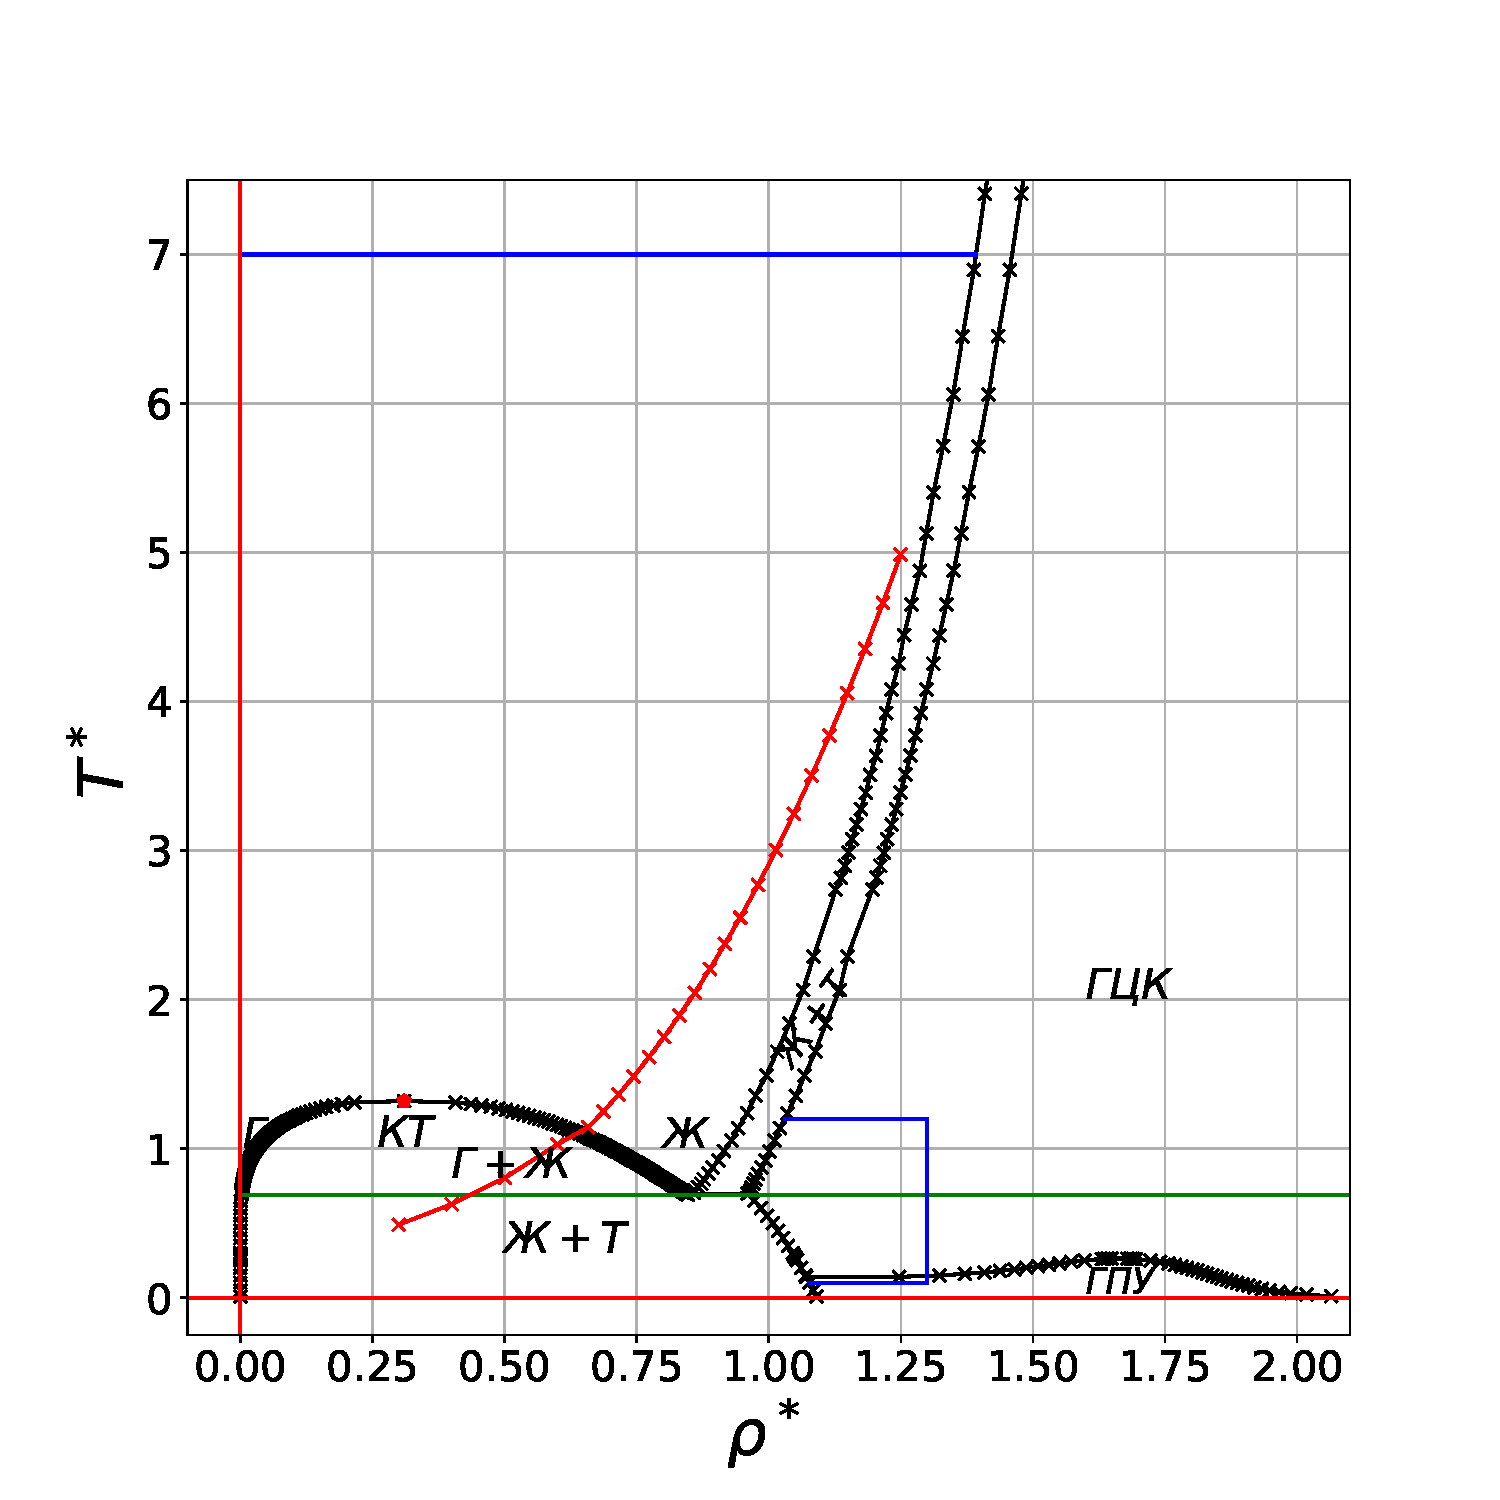
\includegraphics[width=\linewidth]{img/Isontropa.pdf}
    \caption{\label{fig:iso_S} График изоэнтропы на фазовой диаграмме. Основные фазовые состояния вещества: $Г$ $~-$ пар, $Ж$ $~-$ жидкость, \textit{ГЦК/ГПУ} $~-$ кристаллическое состояние вещества с двумя типами решеток (\acrshort{fcc} и \acrshort{hcp}, соответственно). Область \textit{Ж+Т} соответствует области плавления вещества, \textit{Ж+Г}$~-$ области сублимации и \textit{Г+Ж} $~-$ области испарения. Красной точкой \textit{КТ} на графике показана критическая точка, значения плотности и давления в ней равны, соответственно, $\rho_c = 0.31$ и $T_c = 1.32$. Зелёная прямая, проведённая параллельно оси $\rho^*$, показывает значение температуры в тройной точке на фазовой диаграмме, численно равное $T_{triple} = 0.692$. Плотности различных фаз в тройной точке равны, соответственно, $\rho_V = 0.0018$, $\rho_L = 0.847$, $\rho_S = 0.962$ \cite{Baidakov:JETP:2006}. Области на графике, образованные синими прямыми и чёрными кривыми фазовых состояний, показывают границы применимости уравнений состояний для соответствующих фаз.}
\end{figure}

При работе с потенциалом \acrshort{lj} удобно выражать термодинамические величины, такие как температура, плотность, давление и т.д., в безразмерных единицах измерения. Это означает, что необходимо выбрать удобную единицу измерения энергии, длины и массы, а затем получить все другие величины в пересчете на эти базовые единицы измерения. Исходя из записи \acrshort{lj}, естественно за основные принять следующие параметры: $\sigma$ $~-$ единица длины, $\varepsilon$ $~-$ единица энергии, $m$ $~-$ единица массы (масса атомов, участвующих в моделировании). И из этих базовых единиц измерения вытекают все остальные:

\begin{table}[h]
    \caption{\label{tab:table1} Приведённые термодинамические величины \acrshort{lj}}
    \begin{ruledtabular}
        \begin{tabular}{ l l l l }
            Расстояние & $r^* = r/\sigma$ & Энергия & $E^* = E/\varepsilon$\\
            Время & $t^* = t[\varepsilon/(m\sigma^2)]^\frac{1}{2}$ & Температура & $T^* = k_BT/\varepsilon$\\
            Масса & $m^* = m$ & Плотность & $\rho^* = \rho\sigma^3/m$\\
            Сила & $F^* = F\sigma/\varepsilon$ & & \\
        \end{tabular}
    \end{ruledtabular}
\end{table}

Затем из полученного графика было найдено значение плотности в месте пересечения построенной кривой с бинодалью, которое равняется $\rho_{binodal}=0.645$ единицам. Важно отметить данный факт, т.к. в дальнейшем значения плотности вещества за волной разгрузки будут сравниваться с $\rho_{binodal}$, что позволит определить в какой области фазовой диаграммы находится образец: флюидной или двухфазной \textit{Ж+Г}.  